\title{State Machine Analysis}
\begin{document}
\section{State Machine Structure}

\begin{frame}{Clocked synchronous state machines}
  \begin{block}{What is a clocked synchronous state machine?}
    \begin{itemize}
      \item State machine - sequential circuit
      \item Clocked - storage elements are flip-flops
      \item Synchronous - all of the flip-flops use the same clock signal
    \end{itemize}
  \end{block}
  The \alert{state memory} of a state machine is the set of $n$ flip-flops that store the state.
  \begin{itemize}
    \item A state machine with $n$ flip-flops has $2^n$ possible states.
    \item All of the states may not be used.
    \item Often we'll used D flip-flops to represent the state.
  \end{itemize}
\end{frame}

\subsection{Mealy Machine}

\begin{frame}{Mealy machine}
  \begin{center}
    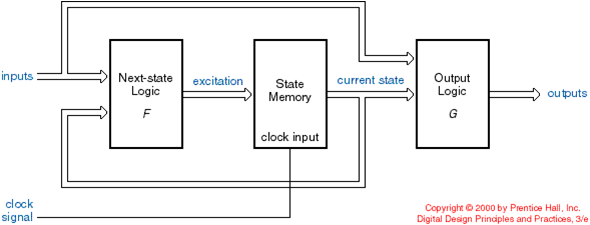
\includegraphics[scale=0.6]{MealyMachine}
  \end{center}
  \begin{block}{Logical Description}
    Next State = F(current state, input)\\
    Output = G(current state, input)
  \end{block}
  Here F and G are combinational circuits.
\end{frame}

\subsection{Moore Machine}

\begin{frame}{Moore machine}
  \begin{center}
    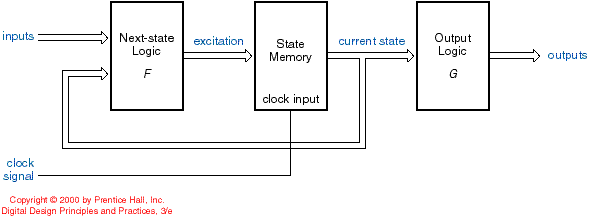
\includegraphics[scale=0.6]{MooreMachine}
  \end{center}
  \begin{block}{Logical Description}
    Next State = F(current state, input)\\
    Output = G(current state)
  \end{block}
  We can have a state machine with Mealy-type or Moore-type outputs, or both.
\end{frame}

\subsection{Characteristic Equations}

\begin{frame}{Characteristic equations}
  \begin{definition}
    A \alert{characteristic equation} is an equation that specifies the next state of a flip-flop or latch in terms of its current state and its inputs.  It is similar to a logic equation.
  \end{definition}
  \begin{center}
    \begin{tabular}{ll}
      S-R latch & $Q* = S + R' \cdot Q$ \\
      D latch & $Q* = D$ \\
      D flip-flop & $Q* = D$ \\
      D flip-flop with enable & $Q* = EN \cdot D + EN' \cdot Q$ \\
      T flip-flop & $Q* = Q'$ \\
      T flip-flop with enable & $Q* = EN \cdot Q' + EN' \cdot Q$ \\
    \end{tabular}
  \end{center}
\end{frame}

\section{State Machine Analysis}

\begin{frame}{Analysis procedure}
  \begin{enumerate}
    \item Determine the excitation equations (combinational input)
    \item Get transition equations from characteristic and excitation equations
    \item Construct a transition table
    \item Assign meaningful state names and construct the state table
    \item Determine the output equations
    \item Construct a state/output table
    \item Draw a state diagram
  \end{enumerate}
\end{frame}

\begin{frame}{State machine analysis example}
  \begin{center}
    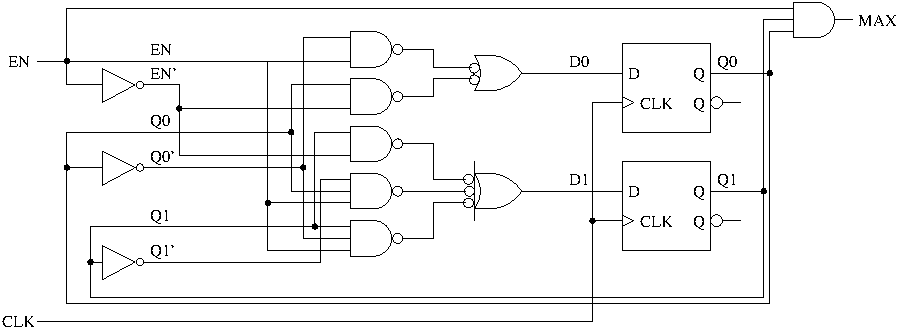
\includegraphics[scale=0.7]{BinaryCounter}
  \end{center}
\end{frame}

\subsection{Logic Equations}

\begin{frame}[t]{Excitation (logic) equations}
  Step 1: Write the logic equations for the combinational input.
\end{frame}

$$D0 = Q0 \cdot EN' + Q0' \cdot EN$$
$$D1 = Q1 \cdot EN' + Q1' \cdot Q0 \cdot EN + Q1 \cdot Q0' \cdot EN$$

\subsection{Transition Equations}

\begin{frame}[t]{Transition equations}
  Step 2: Write the transition equations based on the excitation equations of the combinational input and the characteristic equations of the flip-flops.
\end{frame}

Characteristic equations:
$$Q0* = D0$$
$$Q1* = D1$$

Transtition equations:
$$Q0* = Q0 \cdot EN' + Q0' \cdot EN$$
$$Q1* = Q1 \cdot EN' + Q1' \cdot Q0 \cdot EN + Q1 \cdot Q0' \cdot EN$$

\subsection{Tables}

\begin{frame}[t]{Transition table}
  Step 3: Construct the transition table.
\end{frame}

\begin{tabular}{c|cc}
  Q1 Q0 & Q{0,1}* (EN=0) & Q{0,1}* (EN=1) \\
  \hline
  00 & 00 & 01 \\
  01 & 01 & 10 \\
  10 & 10 & 11 \\
  11 & 11 & 00 \\
\end{tabular}

\begin{frame}[t]{State table}
  Step 4: Assign meaningful state names and construct the state table.
\end{frame}

\begin{tabular}{c|cc}
  S & S* (EN=0) & S* (EN=1) \\
  \hline
  0 & 0 & 1 \\
  1 & 1 & 2 \\
  2 & 2 & 3 \\
  3 & 3 & 0 \\
\end{tabular}

\begin{frame}[t]{Output equations}
  Step 5: Determine the output equations.
\end{frame}

$$MAX = Q1 \cdot Q0 \cdot EN$$

\begin{frame}[t]{State/output table}
  Step 6: Construct the state/output table.
\end{frame}

\begin{tabular}{c|cc}
  S & S*,MAX (EN=0) & S*,MAX (EN=1) \\
  \hline
  0 & 0,0 & 1,0 \\
  1 & 1,0 & 2,0 \\
  2 & 2,0 & 3,0 \\
  3 & 3,0 & 0,1 \\
\end{tabular}

\subsection{State Diagram}

\begin{frame}[t]{State diagram}
  Step 7: Draw the state diagram.
\end{frame}
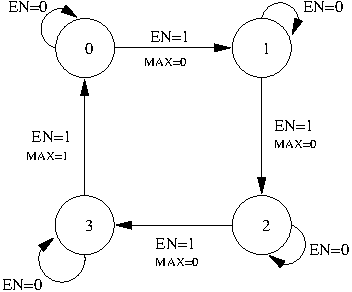
\includegraphics{BinaryCounterStateDiagram}
\end{document}
